\documentclass[12pt]{article}
\usepackage{graphicx}

\usepackage{fontspec}
\usepackage{xunicode}
\defaultfontfeatures{Scale=MatchLowercase}
\setromanfont[Mapping=tex-text]{Optima}

\setlength{\textheight}{8.5in}
\setlength{\evensidemargin}{0.0in}
\setlength{\oddsidemargin}{0.0in}
\setlength{\topmargin}{-0.5in}
\setlength{\textwidth}{6.5in}

%opening
\title{Milestone 2}
\author{Merritt Boyd, Diyang Tang}

\begin{document}

\maketitle

\noindent
\textbf{1. Did any of your previous answers change?}

Yes: 5.  We are probably not going to use all 3 APIs to find search results; given how each gives different information, using fewer would be easier for us and for the user. \\


\noindent
\textbf{2. What feature will you demonstrate to meet the dynamic page generation requirement?}

We will demonstrate searching for a job.  When the user enters a keyword or a location, the site will load a map with markers denoting jobs fitting that keyword or location. \\


\noindent
\textbf{3. Include 1 screenshot demonstrating the feature.}

\begin{figure}[h!]
\centering

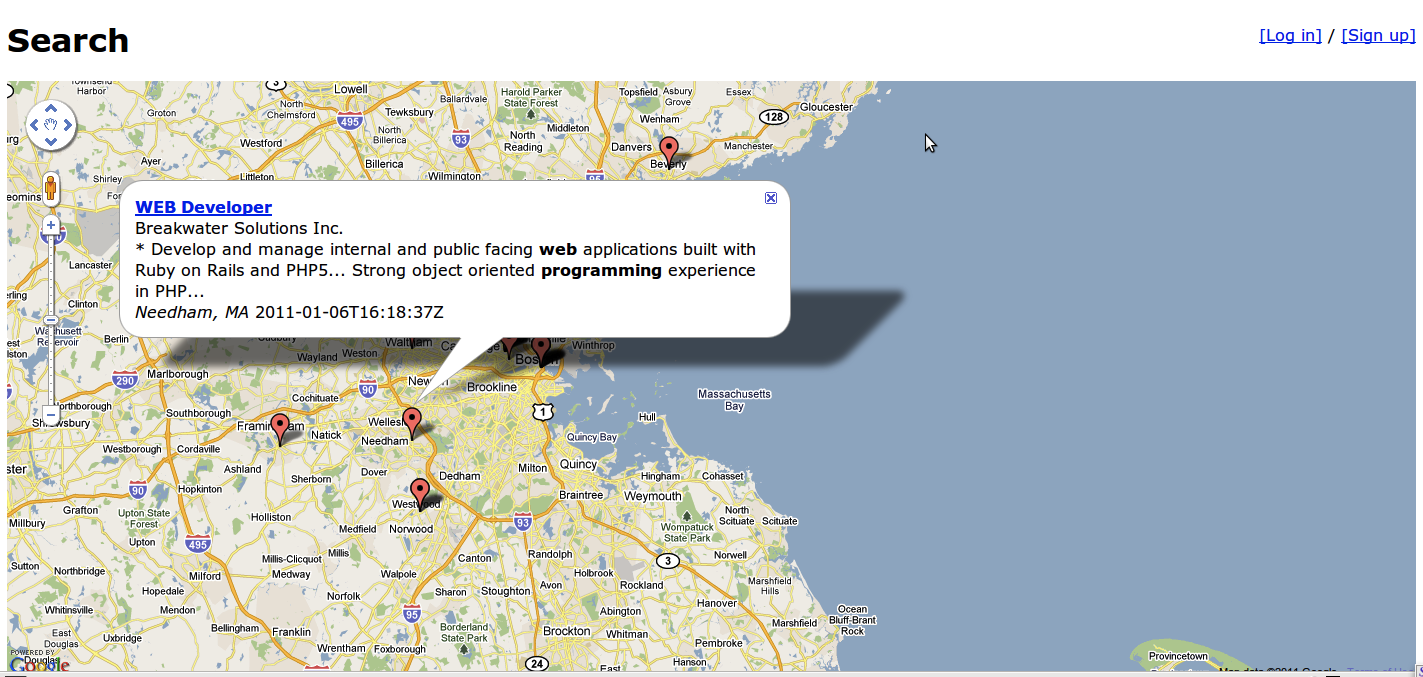
\includegraphics[width=6in]{search.png}
\caption{I searched for ``web programming'' near ``Cambridge, MA'' and received this as a result.}
\end{figure} 

\noindent
\textbf{4. What technology do you plan to use for the front-end?}

We are using HTML5, the Google Maps JavaScript API, Rails' templating engine, and JavaScript libraries such as jQuery. \\

\noindent
\textbf{5. What is the main browser you are targeting?}

We are targeting the latest stable Chrome release. \\

\noindent
\textbf{6. What other features have you already built? Are they necessary for a minimum viable product?}

We have also built user accounts and integrated Facebook and LinkedIn accounts.  They are necessary for a minimum viable product, because without them users cannot import their contacts to see where their contacts have worked. \\

\noindent
\textbf{7. What features do you still have to build for a minimum viable product?}
 
For a minimum viable product, we still need to build a way to import contacts from Facebook and LinkedIn and we need to show that on the same map used to show job query results. \\

\noindent
\textbf{8. What features would you like to build after finishing the core features?}

We would like to: allow advanced searches; make the transition from the home page to the map extremely visually engaging; enable better searching across multiple APIs and with our database; save searches; allow more functionality from the users' imported contacts (for example, help them use their network); and use more attractive markers on the map.\\

\noindent
\textbf{9. What design decision (at any level) are you most proud of?} 

We're most proud of the user-testing with paper prototypes we did for the home page and the map page.  Hopefully this is guiding us to a website that is clear and simple-to-use.  \\

\noindent
\textbf{10. What design decision (at any level) are you least proud of?} 

We're least proud of the fact that our website is minimal not because that was a well-thought-out, deliberate decision, but because we don't have the visual design strength to want a less minimal one.\\

\noindent
\textbf{11. What implementation unknown / risks are you still facing?}

We still have to worry about user interface, design, and search.


\end{document}
